\chapter{Experiments and Discussions}

For the quantification of how well our system works we need some measurements.

\begin{figure}[!htpb]
  \centering
  \caption{Strings Single Note Accuracy}
  \label{single-note-accuracy}
  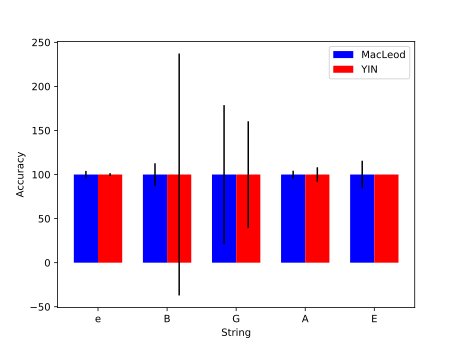
\includegraphics[scale=0.85]{images/measurements/single-note-accuracy}
  \legend{Source: Authors}
\end{figure}

\begin{figure}[!htpb]
  \centering
  \caption{Am Chord Error}
  \label{am-chord-error}
  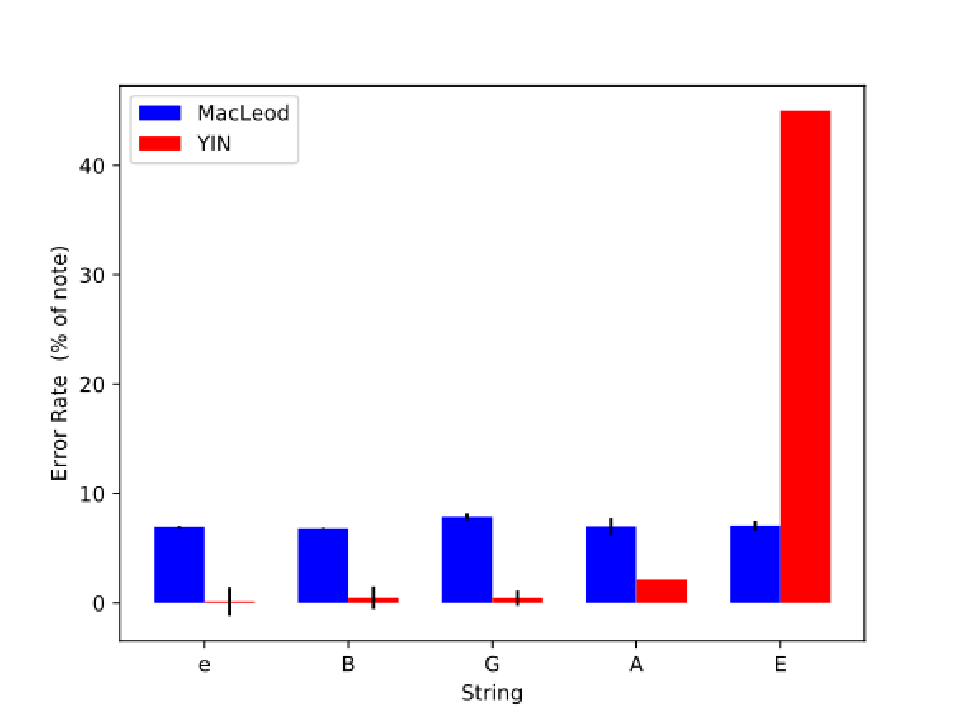
\includegraphics[scale=0.85]{images/measurements/am-chord-error}
  \legend{Source: Authors}
\end{figure}

\begin{figure}[!htpb]
  \centering
  \caption{E Chord Error}
  \label{e-chord-error}
  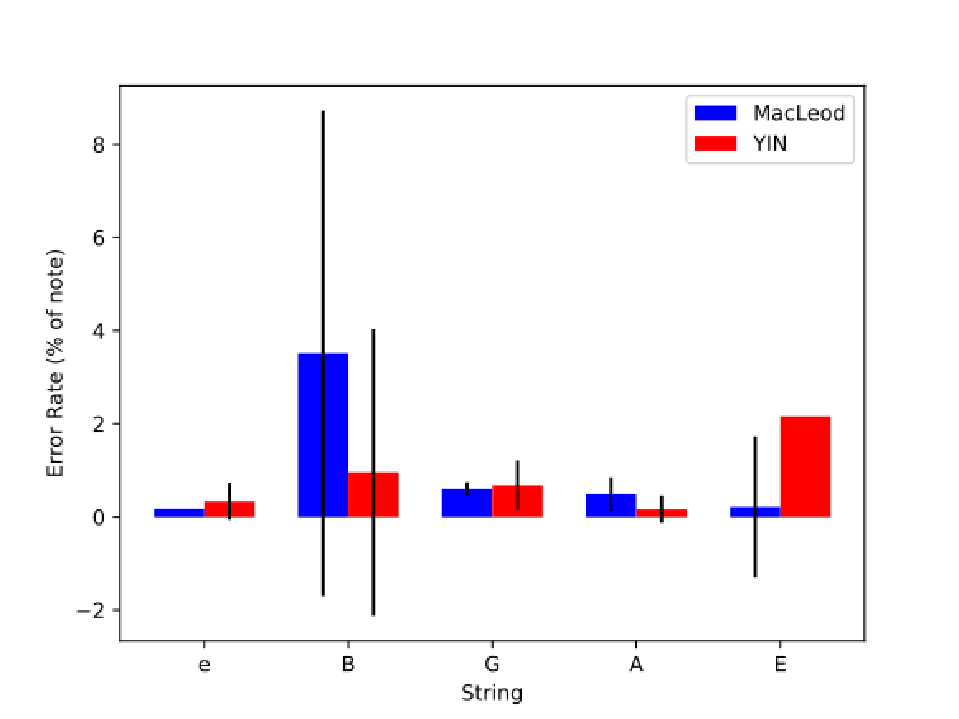
\includegraphics[scale=0.85]{images/measurements/e-chord-error}
  \legend{Source: Authors}
\end{figure}

\section{Discussions}


